\section{Workflow Service}
We are using JPBM (http://www.jboss.com/products/jbpm) as the engine in Workflow
service. Here we demonstrate how this works step by step.
\newline
\newline
After logged in as a curator or administrator, one should have the access to
all the menu items in the Workflow menu, which otherwise only shows Task
Instance and Pending Tasks if your role is the normal user (annotator). After
Click on the Process Definitions link, you will see a list of process
definitions. To add your own process definition, click on the Add button shown
as on the following screenshot.
\begin{center}
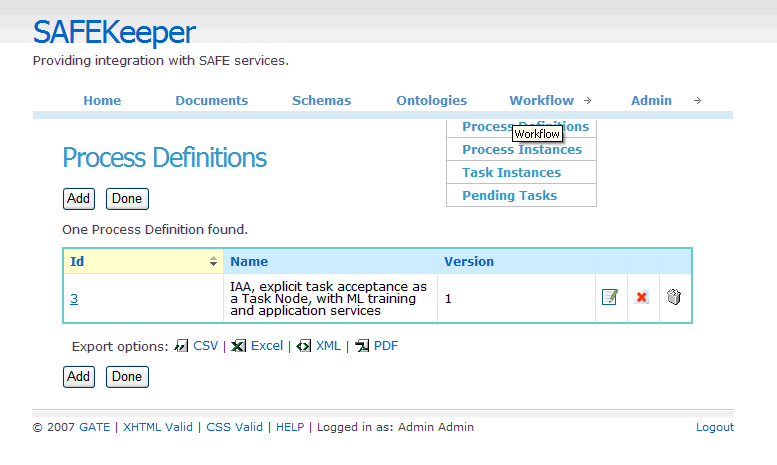
\includegraphics[scale=0.4]{processdefinitionlist}
\end{center}

\begin{figure}[htb]
Then you should reach the Process Definition Upload page, where
you can select your process definition and upload it to the server.
\newline
\newline
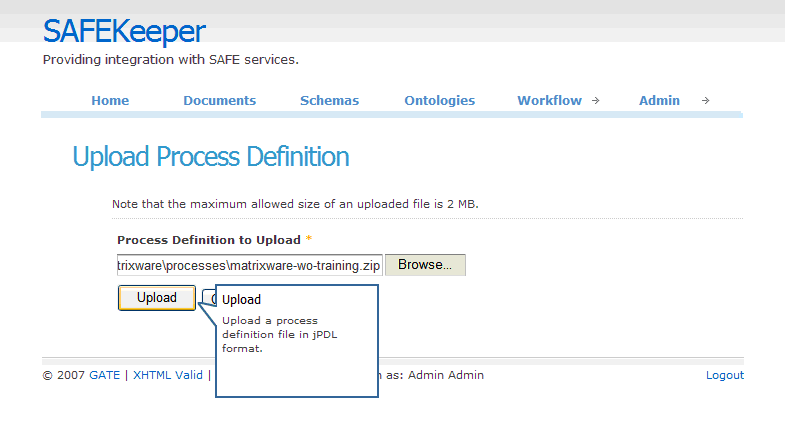
\includegraphics[scale=0.4]{uploadprocessdefinition}
\caption{Process Defintion Upload}
\label{fig:uploadprocessdefintion}
\end{figure}


\begin{figure}[htb]
After uploading successfully and back to the Process Definition 
List page, you should see your newly added process definition. Here 
one can also delete the current version of his process definition 
or all the versions by clicking on the relevant buttons at the end 
of each row in the table.
\newline
\newline
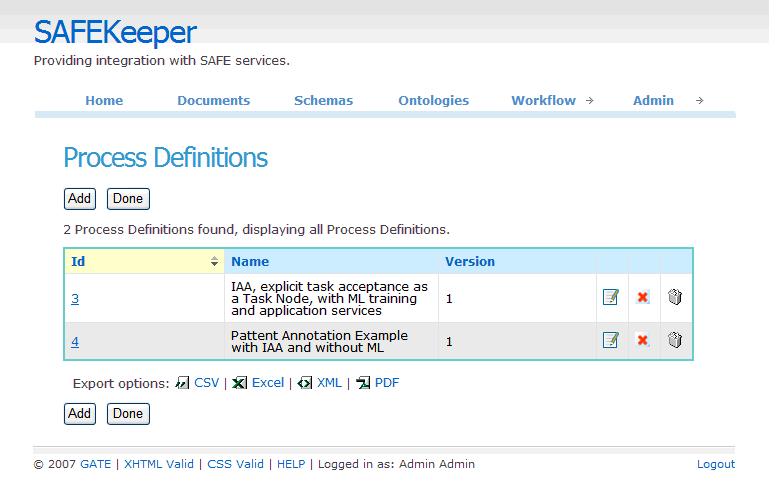
\includegraphics[scale=0.4]{processdefinitionuploaded}
\caption{Added Process Definition}
\label{fig:processdefintionuploaded}
\end{figure}


To view the content of process definition, click on the edit button 
on the above page and then you should see the following page, which 
shows you all the predefined tasks and actors who can be potential 
executors of the tasks (The system remembers the last choices). 
Select actors and click on the button to create the process instance 
and start the process.
\begin{figure}[htb]
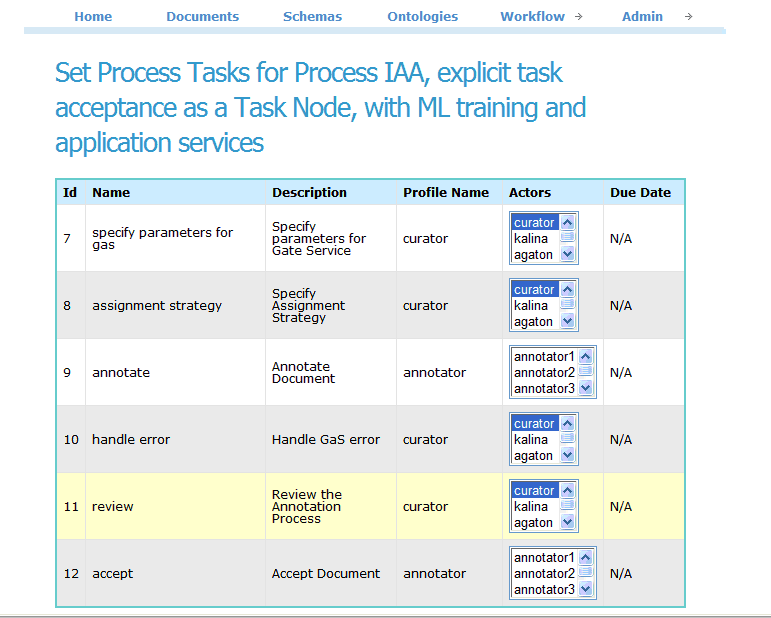
\includegraphics[scale=0.4]{viewprocessdefinition}
\caption{Process Definition View}
\label{fig:viewprocessdefinition}
\end{figure}


To view the started process instances, you can click on the Process
Instance item from Workflow menu. In this stage, you can cancel the 
process by clicking on the crossing button or suspend it.
\begin{figure}[htb]
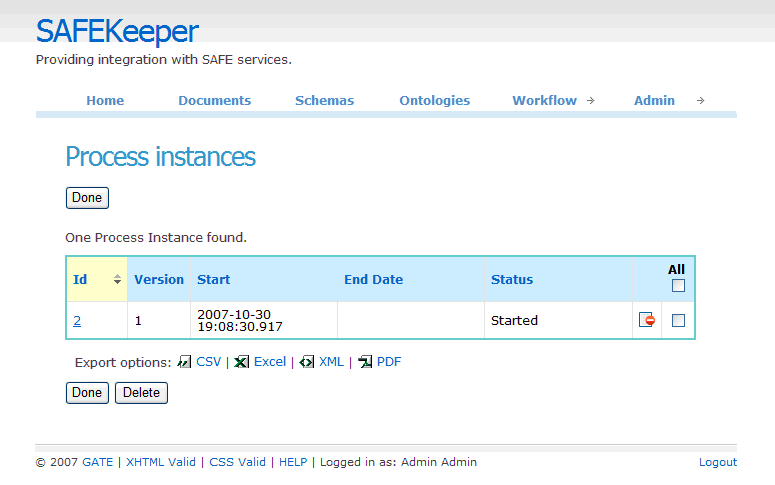
\includegraphics[scale=0.4]{processinstancelist}
\caption{Process Instances}
\label{fig:processinstancelist}
\end{figure}

\begin{figure}[htb]
Now one can see his/her tasks from the Pending Tasks page, in this 
example, the task named “Specify parameters for Gate Service” was 
assigned to curator, so the curator can execute the task by clicking
on the start icon and the icon will disappear if the task is finished.
The following picture shows a list of tasks which include the tasks
either completed or pending.
\newline
\newline
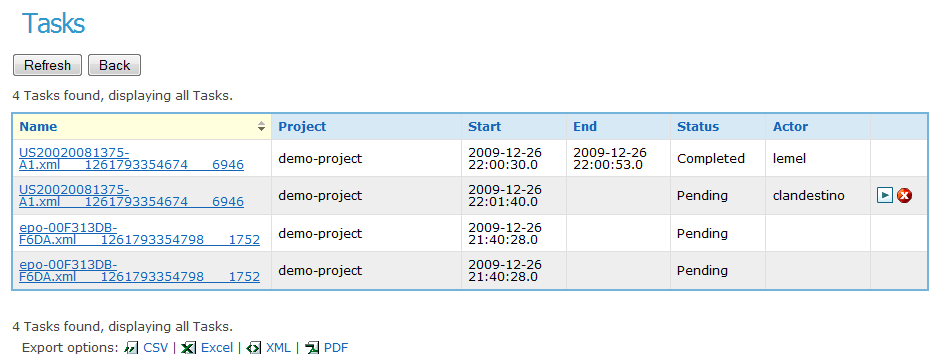
\includegraphics[scale=0.4]{taskinstances}
\caption{Task Instances}
\label{fig:taskinstances}

Once the curator finishes his/her tasks by clicking one of the possible
buttons at the bottom of each task form. Annotators will receive the 
task notification via email, where they can follow the included link to 
launch the Annotator GUI. They can also find their tasks via logging 
into the system and view their pending tasks from the Workflow menu or,
which is more convenient, on the welcome page.
\end{figure}
\newpage
\clearpage
